\section{Introduction}
%Will wrote this introduction - feel free to make changes, but please note the changes too!
The aim of this project was to create a model capable of predicting the sales using information available prior to the launch of a game.

A model capable of making accurate predictions based on several different input parameters would prove quite useful to game development studios trying to anticipate the market performance of a specific project. This model would then also allow said studios to design projects with a mindset of optimising profits. 

The inputs for our model included the price of a game at launch, the genre of the game, the developer and publisher, and whether the game offered additional features e.g. controller support or local multiplayer. Models were then constructed using LASSO, Ridge and kNN Regression, to try and best predict the sales of the given game.

\section{Dataset and Features}
The dataset was prepared...

%Darragh's part
In order to obtain the main dataset that includes the number of sales for different games the SteamSpy API was used. GET requests were sent to the API based on the different genres of games because this would allow us to create a new field for each games list of genres. This was done by interacting with each of the different json files produced from the GET requests and adding the information of each game to a large array within the program. As the games were being stored locally in the program the genres that the game was associated with was also being added to the dictionary. This involved creating a new key in the dictionary and adding the different genres that are associated with each game.

%Will's part
To generate the target feature (the number of sales), a number of features available from SteamSpy had to be manipulated to produce useful values. SteamSpy offered a range of owners to 98\% confidence, but did not offer a precise number of owners for a given game. In a bid to produce better approximations of title ownership, the total number of reviews were normalised between 0 and 1, and then multiplied by the mean of the range in which they resided.
This meant that games with enormous player bases would only normalise against similarly large games, and small games would only be normalised against smaller games.
 
This method then allowed games to have a higher degree of specificity in their ownership, i.e. 200 games which were in the same range of "0 to 20,000" owners could now have weighted, individual numbers of owners assigned to them. This manipulation increased the utility of the target feature.

\section{Methods}
%Will's writing:
Three forms of model were used: LASSO, Ridge and kNN regression in a bid to find which models would best predict the target feature.

Both LASSO and Ridge regression are modifications of Linear regression, in that they each attribute different penalties to the cost functions used to fit their curves.

Taking the cost function of Linear regression to have the form:
\[
J(\theta) = \frac{1}{m} \sum_{i=1}^m (h_{\theta}(x^{(i)}) - y^{(i)})^2
\]

Then $J(\theta)$ for LASSO regression with its (L1) penalty becomes:
\[
J(\theta) = \frac{1}{m} \sum_{i=1}^m (h_{\theta}(x^{(i)}) - y^{(i)})^2 + \frac{1}{C} \sum_{j=1}^n |\theta_j|
\]
And $J(\theta)$ for Ridge regression with its (L2) penalty becomes:
\[
J(\theta) = \frac{1}{m} \sum_{i=1}^m (h_{\theta}(x^{(i)}) - y^{(i)})^2 + \frac{1}{C} \sum_{j=1}^n \theta_j^2
%\frac{\theta^T \theta}{C}
\]

k-Nearest Neighbours regression on the other hand defines weighting based on the proximity between nearby points to make predictions; rather than fitting an overall trend immediately, kNN looks at the local behaviours first to build up a picture of the system. It is in this way that the method is considered "instance-based".
%NEEDS TO BE FINISHED
 Kernelising the kNN involves

\section{Results}

%Will's Part
The results of the investigation fell short of expectations for two chief reasons - the models produced were not of sufficient fidelity for consistently useful predictions, and both the standard and kernelised kNN methods required a prohibitive amount of time to train, preventing the collection of data from those models. %Hold your horses there chief - may be able to do something yet!

These setbacks aside, it was possible to investigate the performance of both the LASSO and Ridge regression methods, by way of mean squared error and $R^2$ value. All models were trained for n=10 splits.
\vspace{8pt}

Figure \ref{fig:fig1} demonstrates why the LASSO model would be thrown out at the earliest convenience. Whilst the mean squared error dips below the baseline at several points, there is no consistent improvement for any values of C. Similarly, all $R^{2}$ values are all less than 0, indicating that the mean is a more accurate prediction than the model.

\begin{figure}[!h]
\begin{small}
\centering
\linespread{1.0}
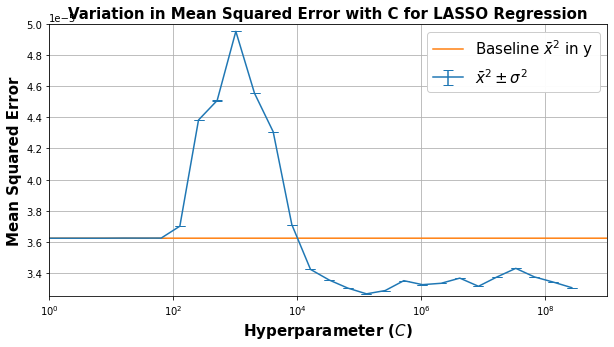
\includegraphics[width=0.8\linewidth]{pics/Lasso_MSE.png}
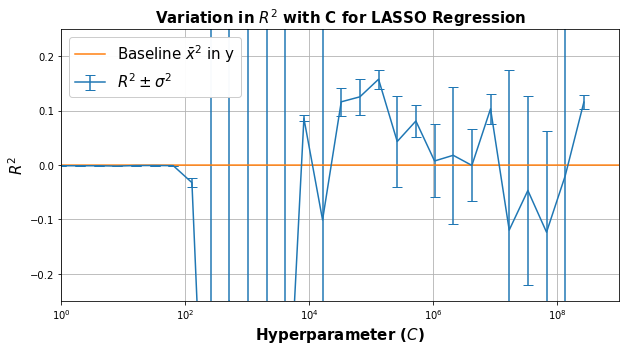
\includegraphics[width=0.8\linewidth]{pics/Lasso_R2.png}
\caption{Varying C has no consistent impact on either MSE or $R^2$.}
\label{fig:fig1}
\end{small}
\end{figure}

Figure \ref{fig:fig2} shows the increased performance of Ridge regression over LASSO regression - MSE is consistently lower for RR, and whilst $R^2$ does fall below zero for increasing C (though $R^2 > 0$ for C $\approx 10$), this is a demonstrable improvement over the LASSO regression. 

\begin{figure}[!h]
\begin{small}
\centering
\linespread{1.0}
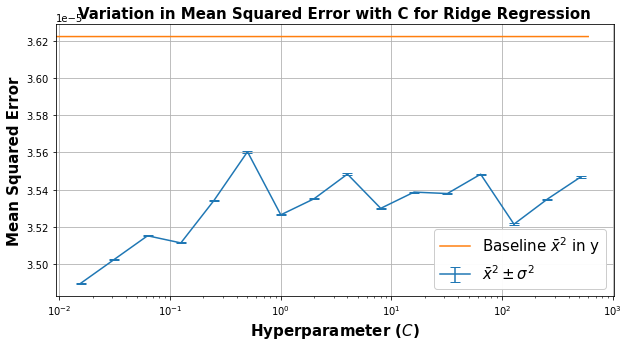
\includegraphics[width=0.8\linewidth]{pics/Ridge_MSE.png}
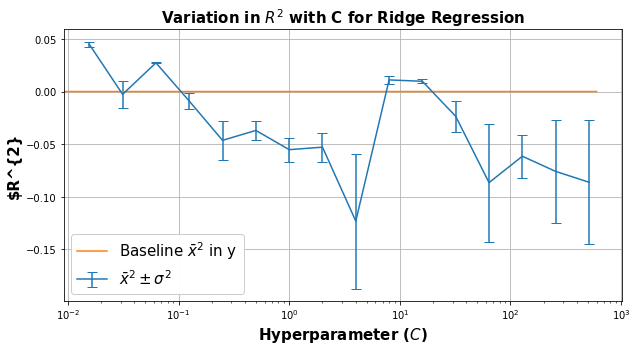
\includegraphics[width=0.8\linewidth]{pics/Ridge_R2.png}
\caption{Increasing C has a negative impact on MSE and $R^2$.}
\label{fig:fig2}
\end{small}
\end{figure}

%Will - "I may have results for kNN soon"

\section{Discussion}

%Darragh's part
One of the hyperparameters that was looked at was the addition of polynomial features. One key issue arose with this which was that due to the high number of parameters the program would run into a memory error, which meant that for this project, polynomial features would not be used.

%Will's part
The aforementioned method of target feature generation used the total number of reviews for a given game to weight the number of owners for a given game. This produced a source of bias towards games that received a higher number of either positive or negative reviews, giving more highly reviewed games more owners. This was deemed an acceptable trade-off against the fact that games may have more actual owners, but who do not leave reviews. As such, the number of owners used as the target feature also reflects the critical engagement of the owners.

\section{Contributions}

Darragh: \\Code contribution - reading in the json files, adding the genres to relevant games and combining all games into one large dicitonary. Attempted to run polynomial features as a hyperparameter.\\ Report contribution - Part of dataset and features, part of discussion

Will:
\\Code contribution - production of the target feature, Y. Training and error analysis of models as found in p\_model.py\\ Report contribution - Template, introduction, part of dataset and features regarding the target feature, methods, results, analysis of results in discussion, analysis of target feature in discussion.